\section{拥塞控制实现}

    \subsection{拥塞控制状态机}
        \subsubsection{基本转换}
        转换如下:
            \begin{figure}[htb]        
                \centering
                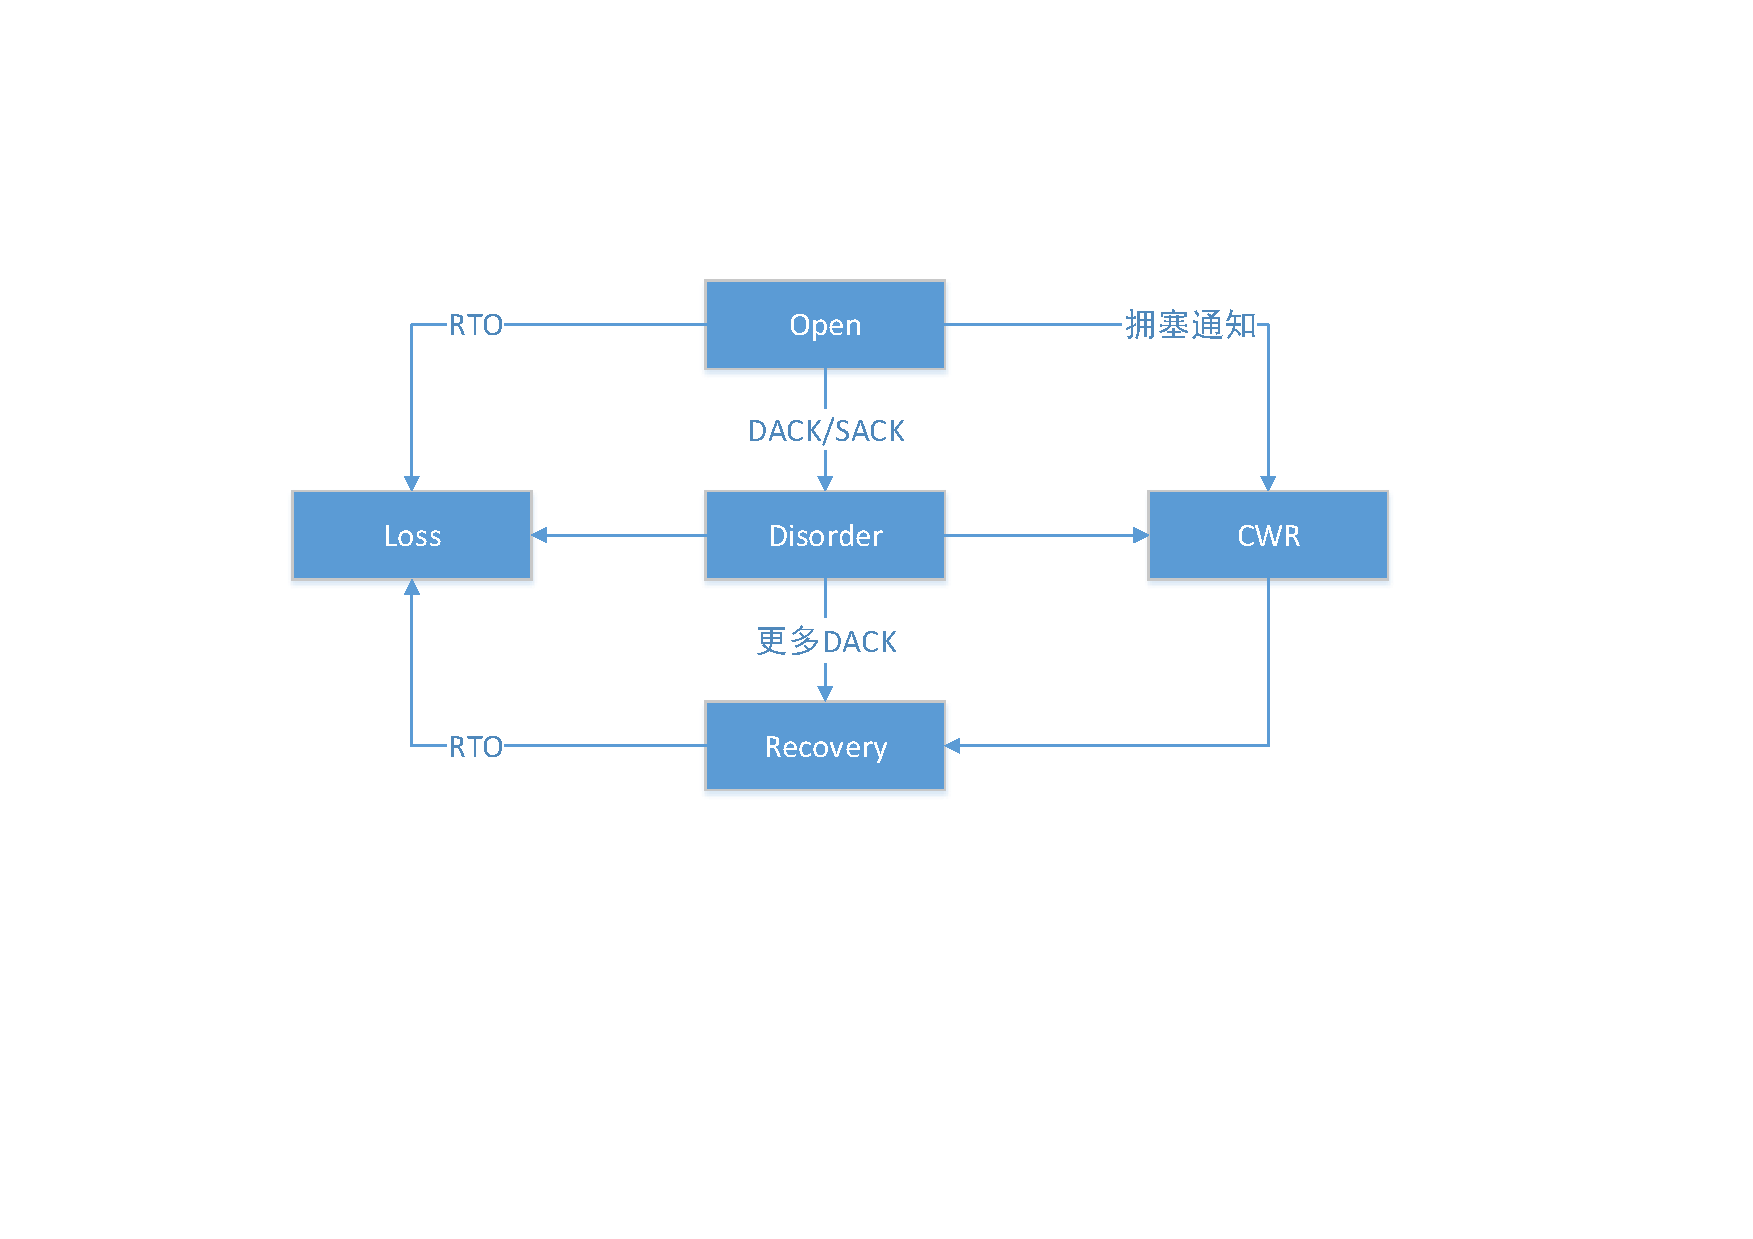
\includegraphics[width=\textwidth]{images/Congestion_Control_State_Machine.pdf}
                \caption{Congestion Control State Machine}
                \label{Congestion Control State Machine}
            \end{figure} 
    
        定义如下:
\begin{minted}[linenos]{C}
enum tcp_ca_state {
    TCP_CA_Open = 0,
#define TCPF_CA_Open    (1<<TCP_CA_Open)
    TCP_CA_Disorder = 1,
#define TCPF_CA_Disorder (1<<TCP_CA_Disorder)
    TCP_CA_CWR = 2,
#define TCPF_CA_CWR (1<<TCP_CA_CWR)
    TCP_CA_Recovery = 3,
#define TCPF_CA_Recovery (1<<TCP_CA_Recovery)
    TCP_CA_Loss = 4
#define TCPF_CA_Loss    (1<<TCP_CA_Loss)
};
\end{minted}
        \subsubsection{Open状态}
            Open状态是常态,在这种状态下TCP发送方通过优化后的快速路径来处理接收ACK。当一个确认到达时,发送方根据拥塞窗口是小于还是大于慢启动阙值,按慢启动或者拥塞避免来增大拥塞窗口。

        \subsubsection{Disorder状态}
            当发送方检测到DACK(重复确认)或者SACK(选择性确认)时,将转变为Disorder(无序)状态。在该状态下,拥塞窗口不做调整,而是每个新到的段触发一个新的数据段的发送。因此,TCP发送方遵循包守恒原则,该原则规定一个新包只有在一个老的包离开网络后才发送。在实践中,该规定的表现类似于IETF的传输提议,允许当拥塞窗口较小或是上个传输窗口中有大量数据段丢失时,使用快速重传以更有效地恢复。

        \subsubsection{CWR状态}
            \label{CongestionState:CWR}
            TCP发送方可能从显式拥塞通知、ICMP源端抑制(ICMP source quench)或是本地设备接收到拥塞通知。当收到一个拥塞通知时,发送方并不立刻减小拥塞窗口,而是每隔一个新到的ACK减小一个段直到窗口的大小减半为止。发送方在减小拥塞窗口大小的过程中不会有明显的重传,这就处于CWR(Congestion Window Reduced,拥塞窗口减小)状态。CWR状态可以被Revcovery状态或者Loss状态中断。进入拥塞窗口减小的函数如下:

\begin{minted}[linenos]{C}
/* 
Location:

    net/ipv4/tcp_input.c

Function:

    Enter CWR state. Disable cwnd undo since congestion is proven with ECN 

Parameter:

    sk:传输控制块
*/
void tcp_enter_cwr(struct sock *sk)
{
    struct tcp_sock *tp = tcp_sk(sk);
    /*进入CWR后就不需要窗口撤消了,
      因此需要清除拥塞控制的慢启动阙值
    */
    tp->prior_ssthresh = 0;
    /*可以看出只有Open状态和Disorder状态可以转移到该状态*/
    if (inet_csk(sk)->icsk_ca_state < TCP_CA_CWR) {
        /*进入CWR状态后不允许在进行拥塞窗口撤消了*/     
        tp->undo_marker = 0;
        /*进行相关的初始化*/
        tcp_init_cwnd_reduction(sk);
        /*设置状态*/        
        tcp_set_ca_state(sk, TCP_CA_CWR);
    }
}
\end{minted}
        关于tcp\_init\_cwnd\_reduction更多的内容,请参见\ref{CongestionControlWindow:tcp_init_cwnd_reduction}。

        \subsubsection{Recovery状态}

            当足够多的连续重复ACK到达后,发送方重传第一个没有被确认的段,进入Recovery(恢复)状态。默认情况下,进入Recovery状态的条件是三个连续的重复ACK,TCP拥塞控制规范也是这么推荐的。在Recovery状态期间,拥塞窗口的大小每隔一个新到的确认而减少一个段,和CWR状态类似。这个窗口减小过程终止与拥塞窗口大小等于ssthresh,即进入Recovery状态时,窗口大小的一半。拥塞窗口在恢复期间不增大,发送方重传那些被标记为丢失的段,或者根据包守恒原则在新数据上标记前向传输。发送方保持Recovery状态直到所有进入Recovery状态时正在发送的数据段都成功地被确认,之后该发送方恢复OPEN状态,重传超时有可能中断Recovery状态。

        \subsubsection{Loss状态}
            \label{CongestionState:Loss}
            当一个RTO到期后,发送方进入Loss状态。所有正在发送的数据段标记为丢失,
            拥塞窗口设置为一个段,发送方因此以慢启动算法增大拥塞窗口。
            Loss和Recovery状态的区别是:Loss状态下,拥塞窗口在发送方设置为一个段后增大,
            而Recovery状态下,拥塞窗口只能被减小。Loss状态不能被其他的状态中断,
            因此,发送方只有在所有Loss开始时正在传输的数据都得到成功确认后,才能退到Open状态。
            例如,快速重传不能在Loss状态期间被触发,这和NewReno规范是一致的。

            当接收到的ACK的确认已经被之前的SACK确认过,这意味着我们记录的SACK信息不能反映接收方的实际状态,
            此时,也会进入Loss状态。

            调用\mintinline{C}{tcp_enter_loss}进入Loss状态,如下:

\begin{minted}[linenos]{C}
/*
Location:

    net/ipv4/tcp_input.c

Function: 
    Enter Loss state. If we detect SACK reneging(违约), forget all SACK information
    and reset tags completely, otherwise preserve SACKs. If receiver
    dropped its ofo?? queue, we will know this due to reneging detection.

Parameter:

    sk:传输控制块

*/
void tcp_enter_loss(struct sock *sk)
{
    const struct inet_connection_sock *icsk = inet_csk(sk);
    struct tcp_sock *tp = tcp_sk(sk);
    struct sk_buff *skb;
    bool new_recovery = icsk->icsk_ca_state < TCP_CA_Recovery;
    bool is_reneg;          /* is receiver reneging on SACKs? */

    /* Reduce ssthresh if it has not yet been made inside this window. */
    if (icsk->icsk_ca_state <= TCP_CA_Disorder ||
        !after(tp->high_seq, tp->snd_una) ||
        (icsk->icsk_ca_state == TCP_CA_Loss && !icsk->icsk_retransmits)) {
        /*保留当前的阙值*/      
        tp->prior_ssthresh = tcp_current_ssthresh(sk);
        /*计算新的阙值*/        
        tp->snd_ssthresh = icsk->icsk_ca_ops->ssthresh(sk);
        /*发送CA_EVENT_LOSS拥塞事件给具体拥塞算法模块*/     
        tcp_ca_event(sk, CA_EVENT_LOSS);
        /*
            在下面的函数中会做以下两个事情:
            tp->undo_marker = tp->snd_una;
            /* Retransmission still in flight may cause DSACKs later. 
                undo_retrans在恢复拥塞控制之前可进行撤销的重传段数???
                retrans_out 重传并且还未得到确认的TCP段的数目
            */
            tp->undo_retrans = tp->retrans_out ? : -1;
        */
        tcp_init_undo(tp);
    }
\end{minted}

    关于tcp\_init\_undo更多内容,请参见\ref{CongestionControlWindowUndo:tcp_init_undo}.

\begin{minted}[linenos]{C}
    /*拥塞窗口大小设置为1*/
    tp->snd_cwnd       = 1;
    /*snd_cwnd_cnt表示自从上次调整拥塞窗口到
     目前为止接收到的总ACK段数,自然设置为0*/
    tp->snd_cwnd_cnt   = 0;
    /*记录最近一次检验拥塞窗口的时间*/
    tp->snd_cwnd_stamp = tcp_time_stamp;
    /*设置重传的但还未得到确认的TCP段的数目为零*/
    tp->retrans_out = 0;
    /*丢失的包*/
    tp->lost_out = 0;
    /*
        查看当前的tp里是否由SACK选项字段,
        有的话,返回1,没有的话返回0
        根据这一点来判断是否需要重置tp中选择确认的包的个数为0
    */
    if (tcp_is_reno(tp))
        tcp_reset_reno_sack(tp);
\end{minted}

    关于tcp\_is\_reno更多的内容,请参见\ref{ACKCheck:IsSACK,IsReno,IsFack};
    关于tcp\_reset\_reno\_sack更多的内容,请参见\ref{ACKUpdate:tcp_reset_reno_sack}.

\begin{minted}[linenos]{C}
    skb = tcp_write_queue_head(sk);
    /*判断接受者是否认为SACK违约*/
    is_reneg = skb && (TCP_SKB_CB(skb)->sacked & TCPCB_SACKED_ACKED);
    if (is_reneg) {
        NET_INC_STATS_BH(sock_net(sk), LINUX_MIB_TCPSACKRENEGING);
        tp->sacked_out = 0;
        tp->fackets_out = 0;
    }
\end{minted}

    关于违约的讲解的更多内容,请参见\ref{TCPFlag}.
\begin{minted}[linenos]{C}
    /*清除有关重传的记忆变量*/
    tcp_clear_all_retrans_hints(tp);

    tcp_for_write_queue(skb, sk) {
        if (skb == tcp_send_head(sk))
            break;

        TCP_SKB_CB(skb)->sacked &= (~TCPCB_TAGBITS)|TCPCB_SACKED_ACKED;
        if (!(TCP_SKB_CB(skb)->sacked&TCPCB_SACKED_ACKED) || is_reneg) {
            /*清除ACK标志*/
            TCP_SKB_CB(skb)->sacked &= ~TCPCB_SACKED_ACKED;
            /*添加LOST标志*/            
            TCP_SKB_CB(skb)->sacked |= TCPCB_LOST;
            /*统计丢失段的数量*/            
            tp->lost_out += tcp_skb_pcount(skb);
            /*重传的最大序号??????*/
            tp->retransmit_high = TCP_SKB_CB(skb)->end_seq;
        }
    }
    /*确认没有被确认的TCP段的数量left_out*/
    tcp_verify_left_out(tp);
\end{minted}

    关于tcp\_verify\_left\_out更多的内容,请参见\ref{WindowCompute:tcp_verify_left_out}。
    
\begin{minted}[linenos]{C}
    /* Timeout in disordered state after receiving substantial DUPACKs
     * suggests that the degree of reordering is over-estimated.
     */
    if (icsk->icsk_ca_state <= TCP_CA_Disorder &&
        tp->sacked_out >= sysctl_tcp_reordering)
        /*重新设置reordering*/
        tp->reordering = min_t(unsigned int, tp->reordering,
                       sysctl_tcp_reordering);
    /*设置拥塞状态*/    
    tcp_set_ca_state(sk, TCP_CA_Loss);
    /*记录发生拥塞时的snd.nxt*/
    tp->high_seq = tp->snd_nxt;
    /*设置ecn_flags,表示发送方进入拥塞状态*/    
    tcp_ecn_queue_cwr(tp);

    /* F-RTO RFC5682 sec 3.1 step 1: retransmit SND.UNA if no previous
     * loss recovery is underway except recurring timeout(s) on
     * the same SND.UNA (sec 3.2). Disable F-RTO on path MTU probing
     */
    tp->frto = sysctl_tcp_frto &&
           (new_recovery || icsk->icsk_retransmits) &&
           !inet_csk(sk)->icsk_mtup.probe_size;
}
\end{minted}

    \subsection{显式拥塞通知(ECN)}
        在处理网络中的拥塞的时候,有一种方法叫做显式拥塞控制。从名字上看就是,
        我们会直接收到关于拥塞的通知。至于是如何实现呢?我这里先简单说一下原理,
        然后再细细说明。当TCP传递的时候,路由器使用IP首部的一对比特位来记录是否
        出现了拥塞。这样,当TCP段到达后,接收方知道报文段是否在某个位置经历过拥塞。
        但是,需要注意的是,发送方才是真正需要了解是否发生了拥塞状况。因此,接收方使用
        下一个ACK通知发送方有拥塞发生。然后,发送方作出响应,缩小自己的拥塞窗口。

        我们知道路由器是网络层的设备,所以说,如果想要路由器帮忙记录拥塞控制就必然需要IP的支持。
        当然,除此之外,也需要TCP层的支持。

        下面是具体的叙述。

        \subsubsection{IP对ECN的支持}

            IP首部中的八位的服务类型域(TOS)原先在RFC791中定义为表明包的发送优先级、时延、吞吐量、
            可靠性和消耗等特征。在RFC2474中被重新定义为包含一个6位的区分服务码点(DSCP)和两个未用
            的位。DSCP值表明一个在路由器上配置的和队列相关联的发送优先级。IP对ECN的支持用到了TOS域的
            剩下的两位。

            基本的定义如下:
\begin{minted}[linenos]{C}
enum {
    INET_ECN_NOT_ECT = 0,   //TOS后两位为00:表示不支持ECN
    INET_ECN_ECT_1 = 1,     //TOS后两位为01:表示支持ECN
    INET_ECN_ECT_0 = 2,     //TOS后两位为10:表示支持ECN??区别
    INET_ECN_CE = 3,        //TOS后两位为11:表示在某路由器处出现拥塞
    INET_ECN_MASK = 3,      //ECN域的掩码
};
\end{minted}


            当路由器检测到拥塞的时候,设置ECN域为11。当然在设置之前会检测之前是否出现了
            拥塞。没有的时候再进行设置。

\begin{minted}[linenos]{C}
/*
Location:

    include/net/inet_ecn.h

Function:


Parameter:

    iph:ip头部。
*/
static inline int IP_ECN_set_ce(struct iphdr *iph)
{
    u32 check = (__force u32)iph->check;        //force???,为啥32位
    u32 ecn = (iph->tos + 1) & INET_ECN_MASK;

    /*
     * After the last operation we have (in binary):
     * INET_ECN_NOT_ECT => 01
     * INET_ECN_ECT_1   => 10
     * INET_ECN_ECT_0   => 11
     * INET_ECN_CE      => 00
     */
    /*不支持ECN的返回0,已经设置拥塞的不重复设置,返回。*/
    if (!(ecn & 2))         
        return !ecn;
    
    /*
     * The following gives us:
     * INET_ECN_ECT_1 => check += htons(0xFFFD)
     * INET_ECN_ECT_0 => check += htons(0xFFFE)
     */
    check += (__force u16)htons(0xFFFB) + (__force u16)htons(ecn);
    
    iph->check = (__force __sum16)(check + (check>=0xFFFF));    //重新计算校验码
    iph->tos |= INET_ECN_CE;    /*把ECN域设置为11,表示发生了拥塞*/
    return 1;
}
\end{minted}

        这里计算校验码需要我们仔细分析一下,remain to do.????
        
        \subsubsection{TCP对ECN的支持}
            路由器使用IP包的相关域来设置相关标志位来表示是否发生了拥塞.而主机使用TCP的首部来告知发送方,网络正在经历拥塞。
            
            TCP使用6位保留位(Reserved)的后两位来支持ECN。两个新的标志CWR、ECE含义如下
\begin{enumerate}
\item[CWR]  CWR为发送端缩小拥塞窗口标志,用来通知接收端它已经收到了设置ECE标志的ACK。
            
\item[ECE]  ECE有两个作用,在TCP三次握手时表明TCP端是否支持ECN;在传输数据时表明接收到的
            TCP段的IP首部的ECN被设置为11,即接收端发现了拥塞.
\end{enumerate}

            当两个支持ECN的TCP端进行TCP连接时,它们交换SYN、SYN+ACK、ACK段。对于支持ECN
            的TCP端来说,SYN段的ECE和CWR标志都被设置了,SYN的ACK只设置ECE标志。

            相关宏定义如下:
\begin{minted}[linenos]{C}
/* 本端支持ECN */  
#define TCP_ECN_OK          1
/* 本端被通知了拥塞,此时作为发送方*/
#define TCP_ECN_QUEUE_CWR   2
/* 通知对端发生了拥塞,此时作为接收方*/
#define TCP_ECN_DEMAND_CWR  4
#define TCP_ECN_SEEN        8
#define TCPHDR_FIN          0x01
#define TCPHDR_SYN          0x02
#define TCPHDR_RST          0x04
#define TCPHDR_PSH          0x08
#define TCPHDR_ACK          0x10
#define TCPHDR_URG          0x20
#define TCPHDR_ECE          0x40
#define TCPHDR_CWR          0x80

#define TCPHDR_SYN_ECN  (TCPHDR_SYN | TCPHDR_ECE | TCPHDR_CWR)
\end{minted}

    \subsection{拥塞控制状态的处理及转换}
        在\label{ClientReceiveSYN+ACK:tcp_ack}章,客户端在第二次连接的时候会调用tcp\_ack
        我们对其分析后,发现其中会调用tcp\_fastretrans\_alert拥塞控制状态处理函数,这里我
        们就主要讲解这一函数。
        \subsubsection{拥塞控制状态处理:\mintinline{C}{tcp_fastretrans_alert}}
            \label{CongestionDeal:tcp_fastretrans_alert}
\begin{minted}[linenos]{C}
/* 
Location:

    net/ipv4/tcp_input.c

Function:

    Process an event, which can update packets-in-flight not trivially.
    Main goal of this function is to calculate new estimate for left_out,
    taking into account both packets sitting in receiver's buffer and
    packets lost by network.
    
    Besides that it does CWND reduction, when packet loss is detected
    and changes state of machine.
    
    It does _not_ decide what to send, it is made in function
    tcp_xmit_retransmit_queue().

Parameter:

    sk:传输控制块.
    acked:得到确认的包的数量
    prior_unsacked:在拥塞控制状态转换之前,从发送队列
                   发出而未得到确认的TCP段的数目.
    is_dupack:是否有重复ACK??需要好好分析分析。
    flag:标志位
*/
static void tcp_fastretrans_alert(struct sock *sk, const int acked,
                  const int prior_unsacked,
                  bool is_dupack, int flag)
{
    struct inet_connection_sock *icsk = inet_csk(sk);
    struct tcp_sock *tp = tcp_sk(sk);
    /**/
    bool do_lost = is_dupack || ((flag & FLAG_DATA_SACKED) && (tcp_fackets_out(tp) > tp->reordering));
    /*means what?????*/ 
    int fast_rexmit = 0;
    /*WARN的返回值是什么呢?
        如果没有待确认的包以及并且选择确认的包的数量不为0,
        就置其为零。
    */
    if (WARN_ON(!tp->packets_out && tp->sacked_out))
        tp->sacked_out = 0;
    /*
        如果选择确认的包的数量为零,并且未确认与已选择确认之间存在段
    */
    if (WARN_ON(!tp->sacked_out && tp->fackets_out))
        tp->fackets_out = 0;
\end{minted}

        接下来,拥塞状态处理机启动。
\begin{minted}[linenos]{C}
    /*  Now state machine starts.
        A. ECE, hence prohibit(阻止) cwnd undoing, the reduction is required. 
        由于接收到显式拥塞通知,因此禁止窗口撤销,并且开始减小拥塞窗口。
    */
    if (flag & FLAG_ECE)
        tp->prior_ssthresh = 0;
\end{minted}

    如果接收到的ACK指向已记录的SACK,这说明我们记录的SACK并没有反应接收方的真实状态。
    也就是说接收方现在已经处于严重的拥塞状态或者在处理上有bug,那么我们接下来就要按照重传超时的方式去处理。
    因为按照正常的逻辑流程,接受的ACK不应该指向已记录的SACK,而应指向SACK并未包含的,这说明接收方由于拥塞已经把
    SACK部分接收的段已经丢弃或者处理上有BUG,我们必须需要重传了。
    
\begin{minted}[linenos]{C}
    /* B. In all the states check for reneging SACKs. */
    if (tcp_check_sack_reneging(sk, flag))
        return;
\end{minted}
    
    关于tcp\_check\_sack\_reneging更多的内容,请参见\ref{TCPACKCheck:tcp_check_sack_reneging}。
    
\begin{minted}[linenos]{C}
    /* C. Check consistency of the current state. */
    tcp_verify_left_out(tp);
\end{minted}

    查看是否从发送队列发出的包的数量是否不小于发出主机的包的数量。
    
    关于tcp\_verify\_left\_out的更多的内容,请参见\ref{WindowCompute:tcp_verify_left_out}.
    
    接下来检测从拥塞状态返回的条件,当high\_seq被确认时,结束拥塞状态,进入Open状态。
\begin{minted}[linenos]{C}
    /* D. Check state exit conditions. State can be terminated
     *    when high_seq is ACKed. */
    if (icsk->icsk_ca_state == TCP_CA_Open) {
        //根据条件判断是否输出警告信息      
        WARN_ON(tp->retrans_out != 0);
        //消除上一次的重传时间戳
        tp->retrans_stamp = 0;
    } else if (!before(tp->snd_una, tp->high_seq)) {
        /*  进入的条件是tp->snd_una>tp->high_seq,即
            拥塞时,记录的SND.NXT被确认了。拥塞情况已经好转很多了。
            此时如果拥塞状态不处于OPen状态,可根据当前的状态结束回
            到Open状态。
        */
        switch (icsk->icsk_ca_state) {
            case TCP_CA_CWR:
                /* CWR is to be held something *above* high_seq
                 * is ACKed for CWR bit to reach receiver. */
                if (tp->snd_una != tp->high_seq) {
                    //结束窗口减小                  
                    tcp_end_cwnd_reduction(sk);
                    //回到OPen状态      
                    tcp_set_ca_state(sk, TCP_CA_Open);
                }
                break;
\end{minted}

    关于tcp\_end\_cwnd\_reduction的更多内容,请参见\ref{CongestionControlWindow:tcp_end_cwnd_reduction}.
\begin{minted}[linenos]{C}
            case TCP_CA_Recovery:
                //判断对方是否提供了SACK服务,提供,返回0,否则返回1
                if (tcp_is_reno(tp))
                    //设置sacked_out为0
                    tcp_reset_reno_sack(tp);
                /*尝试从Recovery状态撤销
                    成功,就直接返回。
                */
                if (tcp_try_undo_recovery(sk))
                    return;
                //结束拥塞窗口缩小
                tcp_end_cwnd_reduction(sk);
                break;
            }
    }
\end{minted}

    关于tcp\_try\_undo\_recovery的更多内容,请参见\ref{CongestionControlWindowUndo:tcp_try_undo_recovery}   ;
    关于tcp\_end\_cwnd\_reduction的更多内容,请参见\ref{CongestionControlWindow:tcp_end_cwnd_reduction}.
    
\begin{minted}[linenos]{C}

    /* Use RACK (Restransmit Ack????)to detect loss 
        有时间好好分析。    
    */
    if (sysctl_tcp_recovery & TCP_RACK_LOST_RETRANS &&
        tcp_rack_mark_lost(sk))
        flag |= FLAG_LOST_RETRANS;//说明重传的丢失

    /* E. Process state. */
    switch (icsk->icsk_ca_state) {
        case TCP_CA_Recovery:
            //判断是否没有段被确认
            if (!(flag & FLAG_SND_UNA_ADVANCED)) {
                //判断是否启用了SACK,未启用返回1,并且收到的是重复的ACK,                
                if (tcp_is_reno(tp) && is_dupack)
                    tcp_add_reno_sack(sk);  //记录接收到的重复的ACK数量
            } else {
                /*确认了部分重传的段*/
                if (tcp_try_undo_partial(sk, acked, prior_unsacked, flag))
                    return;
                /* Partial ACK arrived. Force fast retransmit. */
                do_lost = tcp_is_reno(tp) ||
                      tcp_fackets_out(tp) > tp->reordering;
            }
            if (tcp_try_undo_dsack(sk)) {
                tcp_try_keep_open(sk);
                return;
            }
            break;
\end{minted}

    关于tcp\_add\_reno\_sack的更多内容,请参见\ref{ACKUpdate:tcp_add_reno_sack};
    关于tcp\_try\_undo\_partial的更多的内容,请参见\ref{CongestionControlWindowUndo:tcp_try_undo_partial};
    
\begin{minted}[linenos]{C}
        case TCP_CA_Loss:
            tcp_process_loss(sk, flag, is_dupack);
            if (icsk->icsk_ca_state != TCP_CA_Open &&
                !(flag & FLAG_LOST_RETRANS))
                return;
            /* Change state if cwnd is undone or retransmits are lost */
        default:
            //判断是否开启了SACK,没启用返回1 
            if (tcp_is_reno(tp)) {
                if (flag & FLAG_SND_UNA_ADVANCED)
                    tcp_reset_reno_sack(tp);    //重置sacked
                if (is_dupack)
                    tcp_add_reno_sack(sk);      //记录接收到的sack
            }

            if (icsk->icsk_ca_state <= TCP_CA_Disorder)
                tcp_try_undo_dsack(sk);
            //确定能够离开Disorder状态,而进入Recovery状态。    
            //如果不进入Recovery状态,判断可否进入OPen状态。
            if (!tcp_time_to_recover(sk, flag)) {
                tcp_try_to_open(sk, flag, prior_unsacked);
                return;
            }

            /* MTU probe failure: don't reduce cwnd */
            if (icsk->icsk_ca_state < TCP_CA_CWR &&
                icsk->icsk_mtup.probe_size &&
                tp->snd_una == tp->mtu_probe.probe_seq_start) {
                tcp_mtup_probe_failed(sk);
                /* Restores the reduction we did in tcp_mtup_probe() */
                tp->snd_cwnd++;
                tcp_simple_retransmit(sk);
                return;
            }

            /* Otherwise enter Recovery state */
            tcp_enter_recovery(sk, (flag & FLAG_ECE));
            fast_rexmit = 1;
    }
    //如果接收到重复的ACK或者重传队首的段超时,
    //则要为确定丢失的段更新记分牌
    if (do_lost)
        tcp_update_scoreboard(sk, fast_rexmit);
    tcp_cwnd_reduction(sk, prior_unsacked, fast_rexmit, flag);
    //重传重传队列中那些标记为LOST的段,同时重置RTO定时器。 
    tcp_xmit_retransmit_queue(sk);
}

\end{minted}
